\section{The calculus}


\begin{frame}{The calculus $\Calc$}

  \small

  \begin{itemize}
  \item 
$\Calc$ is inspired by the calculus $\TKGL$ for $\KGL$ presented in
  \citebib{B{\'{\i}}lkov{\'{a}} et al., IJCAR, 2022}.

  \begin{quote}
  \medfont  $\KGL$: extension of     $\GWCL$, over a more expressive language
(involutive negation,   co-implication)

\end{quote}
  


    

 \item 
   $\Calcc$ is a generalization of the calculus %$\Calcc$
   for the logic $\GWCL$ introduced
   in  \citebib{Ferrari et al., TABLEAUX, 2025}.
  
  \end{itemize}
  

  
  \BSK

  \tb{$\Calc$ is refutation calculus} acting on constraints over
  labelled formulas (labels representing worlds of G\"odel-Kripke models).
  
  \MSK
  
  \bfb{Results overview}
  \begin{itemize}\small
  \item termination
  \item completeness
  \item countermodel-construction and finite model property
  \item proof-search procedure (no-backtracking)\\
  \item PSPACE-decidability 
  \item JTabWb implementation
  \end{itemize}
    
  \VFILL
\end{frame}

%=============================================================================

\begin{frame}
  \frametitle{The calculus $\Calc$: constraints}

  \begin{center}
    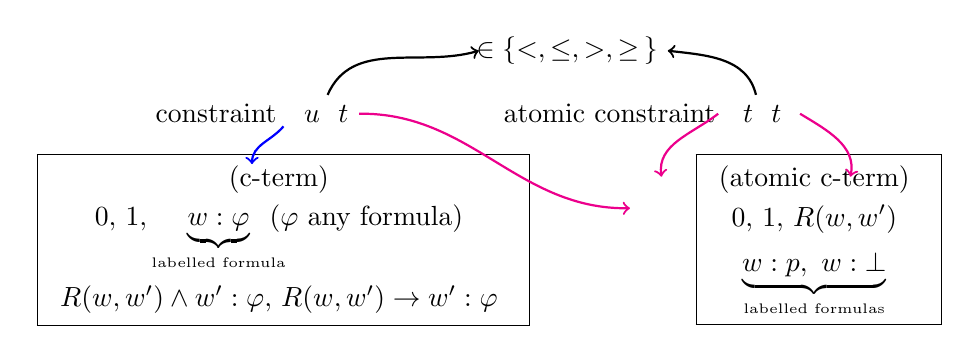
\begin{tikzpicture}[scale=0.8]

      %% ABSTRACT_ORDER
      \draw (3,1) node{
        \medfont \mbox{$\abstractorder\in \{<,\leq,>,\geq\,\}$}
      };

      %% CONSTRAINT
      \draw (-2,0) node{
        \mbox{\tb{constraint}\quad$\tb{u}~\abstractorder~\tm{t}$}
      };

      %% ATOMIC CONSTRAINT
      \draw (4.2,0) node{
        \mbox{\tm{atomic constraint}\quad$\tm{t}~\abstractorder~\tm{t}$}
      };

      %% C-TERM
      \draw (-1.5,-2) node{
        \framebox{\medfont 
          $
          \begin{array}{c}
            \mbox{\tb{(c-term)}}
            \\[.5ex]
            0,\, 1,\underbrace{\tb{w:\varphi}}_{\mbox{\tiny labelled formula}}\hspace{-2.5ex}~
            \mbox{(\tb{$\varphi$ any formula})}
            \\[4ex]
            R(w,w')\land w':\varphi,\, R(w,w')\to w':\varphi
          \end{array}
          $
        }
      };

      %% ATOMIC_C-TERM
      \draw (7,-2) node{
        \framebox{\medfont 
          $
          \begin{array}{c}
            \mbox{\tm{(atomic c-term)}}
            \\[.5ex]
            0,\,1,\, R(w,w')
            \\[1ex]
            \underbrace{\tm{w:p}, ~\tm{w:\bot}}_{\mbox{\tiny labelled formulas}}
          \end{array}
          $
        }
      };

      %%%%%%%%%%%%%%%%%%%%% ARROWS
      %% from CONSTRAINT to ABSTRACT_ORDER
      \draw[thick,->] (-0.8,.3) to[out=50,in=-180,relative] (1.6,1);
      %% from ATOMIC_CONSTRAINT to ABSTRACT_ORDER
      \draw[thick,->] (6,.3) to[out=-50,in=-160,relative] (4.6,1);
      %% from CONSTRAINT left to C-TERM
      \draw[blue,thick,->] (-1.5,-.2) to[out=0,in=-140,relative] (-2,-.8);
      %% from CONSTRAINT right to ATOMIC_C-TERM
      \draw[magenta,thick,->] (-.3,0) to[out=20,in=200,relative] (4,-1.5);
      %% from ATOMIC_CONSTRAINT right to ATOMIC_C-TERM
      \draw[magenta,thick,->] (6.7,0) to[out=20,in=130,relative] (7.5,-1);
      %% from ATOMIC_CONSTRAINT left to ATOMIC_C-TERM
      \draw[magenta,thick,->] (5.4,0) to[out=-10,in=-130,relative] (4.5,-1);
      
    \end{tikzpicture}
  \end{center}


  \MSK
  
  \bfb{Examples}

  
  \begin{center}\medfont
    \begin{tabular}{p{30ex}|p{50ex}}
      \emb{Constraint} & \emm{Intuitive semantical reading}\\[4ex]
   (1) \; $w_0 : \a \;\tm{<}\; w_1 : p $ & The value of formula $\a$ at world $w_0$  is \tm{$<$} than the value of  $p$ (prop.~var.) at world $w_2$ 
      \\[4ex]
      %%%%%%%%%%
     (2)\; $w_0 :\a \;\tm{\geq}\; R(w_0,w_1)  $  &
       The value of formula $\a$ at world $w_0$  is \tm{$\geq$} than the value of  $R(w_0,w_1)$
      \\[4ex]  
      %%%%%%%%%%
     (3)\; $ R(w_0,w_1) \to \tm{\underbrace{\black w_1: \a}_{\tm{r}}}  \;\tm{>}\; 0$ 
      &
Let $\tm{r}$ be the  the value of $\a$ at $w_0$.\\[-2.5ex]
     &   The value of   $ R(w_0,w_1) \to \tm{r}$      is \tm{$> 0$}
    \end{tabular}
  \end{center}
  
  \VFILL
\end{frame}

%=============================================================================

\begin{frame}
    \frametitle{The calculus $\Calc$: constraints}


%  \small
    Let  $\G$ be a set of constraints and  $\M=\stru{W,R,e}$ be a model.

 \begin{center}
    \begin{tcolorbox}[colframe=blue!75!black,width=30em]
      \center
    \bfb{$\Mcal\models \G$  ($\Mcal$ satisfies $\G$)} iff:
      \begin{itemize}
      \item  there exists an  interpretation
  $\iota$  mapping each world label in $\G$ to a world in $W$
  such that
  $\iota(u)\abstractorder\iota(t)$ for every constraint $u\abstractorder t\in\G$\\    
        
\end{itemize}
\emm{All constraints are
    simultaneously satisfied in  $\M$ under $\iota$}. 
    \end{tcolorbox}
  \end{center}
    
  



  \MSK

  \bfb{Example}
  \[
  \tb{\G}\;=\;\{\; \ycbox{$w':\Box p \;\tr{<}\; w'':q$}\,,\;\ggbox{$w'':p\land q \;\tr{>}\; w':p$}\;\}
  \]
  \vspace{-5ex}
  \begin{center}
    \begin{tabular}{p{45ex}p{20ex}}
    \begin{minipage}{45ex}
    \begin{tikzpicture}[scale=0.8]      
      % WORLDS  
      % w0
      \draw[fill] (0,-0.5) circle (3pt)
      +(0,-0)   node (w0)  {}  % used to label the circle 
      +(0,-0.3) node  {\worldsfont $w_0$}
      +(1,0) node  {
        \begin{minipage}{10ex}\worldsfont
          \[
          \begin{array}{l}
            p=0.1\\[1ex]
            \tb{\Box p=0.3}
          \end{array}
          \]
        \end{minipage}
        }
      ;
      
      % w1 
      \draw[fill]  (-2,1) circle (3pt)
      +(0,0)   node (w1)  {}  % used to label the circle 
      +(-0.6,0)  node  {\worldsfont $w_1$} 
      +(0,.8) node  {
        \begin{minipage}{10ex}\worldsfont
          \[
          \begin{array}{r}
            p=0.7
          \end{array}
          \]
        \end{minipage}
        }
      ;
            
      % w2
      \draw[fill] (2,1) circle (3pt)
      +(0,0)   node (w2)  {}  % used to label the circle 
      +(-0.6,0) node{\worldsfont $w_2$}
      +(-.2,.8) node{
        \begin{minipage}{10ex}\worldsfont
          \[
          \begin{array}{l}
            p=0.3, q=0.5\\
            \tb{p\land q=0.3}
          \end{array}
          \]
        \end{minipage}
        }
      ;

\draw(-1,-1) node{$\tb \M$};
      
      % ARROWS
      \draw[magenta,->] (w0) -- (w1) node[midway,above, xshift=-1em,yshift=-2ex] {\worldsfont 1}; 
      \draw[magenta,->] (w0) -- (w2)  node[midway,below, xshift=.5em,yshift=+0.5ex] {\worldsfont 1};  
    \end{tikzpicture}
        \end{minipage}
    &
      \begin{minipage}{6em}
    \small    \tb{Interpretation $\iota$}
      $
      \begin{array}{rcl}
        w'&\mapsto&\tm{w_0}\\
        w''&\mapsto&\tm{w_2}\\
      \end{array}
      $

      \vspace{2ex}
      $\tb{\M\models\G}$
    \end{minipage}
    \end{tabular}
  \end{center}


  \VFILL

  
\end{frame}

% ===================================================================================

\begin{frame}
  \frametitle{The calculus $\Calc$: soundness}
  
  $\Calc$ is a \emm{refutation calculus for constraint sets $\G$}, namely:

  \SSK

  \bfb{Soundness}  
  \begin{center}
    \begin{tcolorbox}[colframe=blue!75!black,width=30em]
      \center
      $
      \provesgw{\Gamma}
      \quad \tr{\Rightarrow}\quad
      \mbox{there is no $\GWL$-model $\M$ s.t.}~\M\models\G
      $
    \end{tcolorbox}
  \end{center}

  %\begin{theorem}[Soundness]
  %  If $$, then $\M\not\models\G$, for every $\M$.
  %\end{theorem}
  
  \SSK

  {\small
    \begin{tcgreenbox}{Application}
    \vspace{-2ex}
    \[
    \begin{array}{c}
      \mbox{%If we can build a derivation for the constraint
      $\provesgw $  \ycbox{$w_0:\varphi<1$}}
      \\[1ex] 
      \tr{\Downarrow}
      \\[1ex] 
        \mbox{there is no $\M$ s.t. $\M\models \ycbox{$w_0:\varphi <1$}$}\\
        \tr{\Downarrow}
        \\[1ex] 
      \tb{\forall\,\M\,,\,\forall\,w\in\M}~e(w,\varphi)=1
      \\[.5ex]
      \text{\blue\em\scriptsize \emph\ no $\GWL$-countermodel for $\varphi$}
        \\[1ex]        %\tb{\forall\,\M}=\stru{W,R,e}~\mbox{and}~\t5b{\forall\,w}\in W~\tb{e(w,\varphi)=1}\\
        \tr{\Downarrow}
        \\[1ex]
        \varphi\in\GWCL
    \end{array}
    \]
    \vspace{.5ex}
  \end{tcgreenbox}
  }

  
  
  \VFILL
\end{frame}

%================================================================================

\begin{frame}
  \frametitle{The calculus $\Calc$: some rules}


  Rules of the calculus, read bottom-up, must decompose a non-atomic constraint in a sound way

  \medskip
  {\blue\bf Rules for $\land$-constraints}
  \[
e(w,\, \a \,\tr{\land}\, \b)\;=\; e(w,\a)\;\tr{\land}\;e(w,\b)\;=\;\tr{\min}\{\; e(w,\a)\,,\,e(w,\b)    \;\}
    \]
   
    
  
  \[\small
    \begin{array}{c}
      \small
      %% AND >
    \AXC{$\ycbox{$w: \a \;\tm{>}\; t$},\;  \ycbox{$w: \a \;\tm{>}\; t$},   \, \G$}   
    % ------------------------------------------      
    \RightLabel{$\tr{\land >}$}
    \UIC{$\ggbox{$w: \a\land \b\; \tm{>}\; t$},\,\G$}
    \DP
      \\[4ex]
    e(w,\a \land \b) > t \quad\tr{\Implies}\quad  e(w,\a) > t\;\tr{\land }\;  e(w,\b) > t
      \\[6ex]
  %=============================================================    
    %% AND < 
    \AXC{$\ycbox{$w: \a \;\tm{<}\; t$},\, \G$}   
    \AXC{$\ycbox{$w: \b \;\tm{<}\; t$},\, \G$}
    % ------------------------------------------      
    \RightLabel{$\tr{\land <}$}
    \BIC{$\ggbox{$w: \a\land \b\; \tm{<}\; t$},\,\G$}
      \DP
        \\[4ex]
    e(w,\a \land \b) < t \quad\tr{\Implies}\quad  e(w,\a) > t\;\tr{\lor }\;  e(w,\b) > t
      \end{array}
    \]

    \smallskip
    The rules concerning the other propositional connectives are similar 
\end{frame}  

%================================================================================

\begin{frame}
  \frametitle{The calculus $\Calc$: rules}

 {\blue\bf Rule for $\Box$-constraints}

 \[ 
 e(w, {\Box} \a) = {\tr\inf}\ \Big\{\,R(w,{x})\,{\to}\, e(x,\a)~|~w\in W\,\Big\}
      %\quad $e(w, {\Diam} \a)= {\sup}_{{x}\in W}\Big\{\,R(w,{x})\, {\land}\, e(x,\a)\,\Big\}$
 \]
 
      \smallskip
 Let   $e(w, \Box \a)=\tm r$. The value $\tm r$ is witnessed by a world $\tb{w_1}$, namely: 
\[\small
  R(w,\tb{w_1}) \to \tb{w_1}: \a \,=\,\tm r   
\]
  


  
  \[\small
    %% BOX <
    \AXC{$\ycbox{$\overbrace{R(w,\tb{w_1}) \to \tb{w_1}: \a}^{\tm r} \;\tm{<}\; t$},\;  \ycbox{$\Phibd{\G,w,\tb{w_1}}$},   \, \G$}   
    % ------------------------------------------      
    \RightLabel{$\Box\tm{<}$}
    \UIC{$\ggbox{$\underbrace{w: \Box \a}_{\tm r}\; \tm{<}\; t$},\,\G$}
    \DP\qquad \text{$\tb{w_1}$ new}
    \]

  \[\medfont
       \begin{array}{lcl}
         \Phibd{\G,w, w_1} &\,=\,&
                                   \{\, R(w,w_1)\to w_1: \b \gt\!' t~|~w :\Box \b\gt\!' t \in\G  \,\}\,\cup\,
                                   \\[1ex]
         &&\{\, R(w,w_1)\land w_1: \b \lt\!' t~|~w :\Diam \b\lt\!' t \in\G  \,\}
          \\[1ex]
         && \lt,\lt'\in\{<,\leq\},\; \gt,\gt'\in\{>,\geq\}.
       \end{array}
       \]
       No rule for constraints of the form
       \[
w: \Box \a > t \qquad w: \Box \a \geq t
       \]
\end{frame}  


%==================================================================

\begin{frame}
  \frametitle{The calculus $\Calc$: axioms}\small


  \begin{tcgreenbox}[top=0ex]{}
    A set of atomic constraint \bfb{$\Gat$ is consistent} if we can
    define a function \tm{$\s$} mapping:
    \[
        \tb{\fbox{$w:p$}}\mapsto q\in\Qrange\quad \tb{\fbox{$R(w,w')$}}\mapsto q\in\Qrange\quad \tb{w:\bot}\mapsto 0
    \]
    so that \emm{all constraints in $\s(\Gat)$ are simultaneously satisfied}.
    %% for every $u\abstractorder t\in\Gat$,
    %% $\s(u)\abstractorder\s(t)$ holds ().
  \end{tcgreenbox}

  \SSK

  \bfb{Examples}
  \begin{itemize}
  \item \medfont
\[
    \G= \{\ycbox{$w_1 : p$} > \gcbox{$R(w_1,w_2)$},\, \ggbox{$w_2 : p$} \leq \gcbox{$R(w_1,w_2)$},\,
    \gcbox{$R(w_1,w_2)$} < 1,\,  \ggbox{$w_2 : p$} > \underset{\tm 0}{w_1 :\bot}   \,\}
  \]
  is consistent. Indeed, let:
    \[
    \tm{\s}: \ycbox{$w_1:p$}\mapsto 0.8\,,\,
    \gcbox{$R(w_1,w_2)$}\mapsto 0.6\,,\,
    \ggbox{$w_2:p$}\mapsto 0.4\,,\,
    \]
    \[
      \G= \{\underset{\tm{0.8}}{\ycbox{$w_1 : p$}} > \underset{\tm{0.6}}{\gcbox{$R(w_1,w_2)$}},\,
      \underset{\tm{0.4}}{\ggbox{$w_2 : p$}} \leq \underset{\tm{0.6}}{\gcbox{$R(w_1,w_2)$}},\,
    \underset{\tm{0.6}}{\gcbox{$R(w_1,w_2)$}} < 1,\,  \underset{\tm{0.4}}{\ggbox{$w_2 : p$}} > \underset{\tm 0}{w_1 :\bot}   \,\}
  \]

    
    
    \MSK
    
  % \item $\G=\{w : \Box \a > w':p, w':0 \leq 1, w':p \geq 1\}$ is not consistent,
  %   Indeed $\Atmp{\G} = \{1 > w':p,w':p \leq 1,w':p \geq 1\}$ cannot be
  %   satisfied.  Note that with $\tm{\s}:w':p\mapsto 1$ $\s(\Atm{\G})$ is
  %   satisfied, but there is no model satisfying $w : \Box \a >1$ (and
  %   hence no model satisfying $\G$).

  \end{itemize}

  % \MSK

  
  % \emb{Consistency of $\Gat$ can be checked by a Constraint Solver
  % over $\mathbf{Q}$}.

  % \SSK

  % An atomic labelled formula \fbox{$w:p$} can be considered as a
  % constant name.


  \VFILL
\end{frame}



%================================================================================

\begin{frame}{The calculus: axioms}


  

  \small
  \[
     %% AXAT 
    \AXC{}
    \RightLabel{\small$\ruleAxat$}
    \UIC{$\G$}    
    \DP\quad\mbox{if $\Atmp{\G}$ is not consistent}
 \]
The side condition guarantees that there is no model $\M$ such that $\M\models \G$.
  
\[
    \mbox{\medfont $\Atmp{\G}=\Atm{\G}\bigcup
      \underbrace{ %
        \{\tb{1} > t\,|\,\tb{\fbox{$w : \Box \a$}} > t \in \G\,\}
        \cup
        \{\tm{0} < t\,|\,\tm{\fbox{$w : \Diam \a$}} < t \in \G\,\}
        }_{\mbox{needed to guarantee the coherence}}$}
   \]

  %(1) and (2) are needed to guarantee the coherence of the assignment
  %in a model.

  \vspace{10ex}
  

  \bfb{Example}
  \[
    \begin{array}{rcl}
      \G_0 &=&\{\,w_0 : \Box p_0 > w_1:p_1,\, w_1:p_1 \leq 1,\, w_1:p_1 \geq 1\,\}
   \\[1ex]          
      \Atmp{\G_0}& =  & \{\,1 > \ggbox{$w_1:p_1$},\,\ggbox{$w_1:  p_1$} \leq 1,\, \ggbox{$w_1:p_1$} \geq 1\,\}
\qquad\text{\red not consistent}
    \end{array}
  \]
  \begin{itemize}
  \item $\G_0$ is an initial constraint set

\item There is no  model $\M$ such that $\M\models \G_0$
  \end{itemize}



  \MSK

  
  \emb{Consistency of $\Gat$ can be checked by a Constraint Solver
  over $\mathbf{Q}$}.

  \SSK

  Formulas \fbox{$w:p$} and s \fbox{$R(w_1,w_2)$}  can be abstracted by variables
  



  \VFILL
\end{frame}


%==================================================================

% \begin{frame}
%   \frametitle{The calculus: axioms}\small


%   \begin{tcgreenbox}[top=0ex]{}
%     A set of atomic constraint \bfb{$\Gat$ is consistent} if we can
%     define a function \tm{$\s$} mapping:
%     \[
%         \tb{\fbox{$w:p$}}\mapsto q\in\Qrange\quad \tb{\fbox{$R(w,w')$}}\mapsto q\in\Qrange\quad \tb{w:\bot}\mapsto 0
%     \]
%     so that \emm{all constraints in $\s(\Gat)$ are simultaneously satisfied}.
%     %% for every $u\abstractorder t\in\Gat$,
%     %% $\s(u)\abstractorder\s(t)$ holds ().
%   \end{tcgreenbox}

%   \SSK

%   \bfb{Examples}
%   \begin{itemize}

    
%    \item $\G=\{w : \Box \a > w':p, w':0 \leq 1, w':p \geq 1\}$ is not consistent,
%      Indeed $\Atmp{\G} = \{1 > w':p,w':p \leq 1,w':p \geq 1\}$ cannot be
%      satisfied.  Note that with $\tm{\s}:w':p\mapsto 1$ $\s(\Atm{\G})$ is
%      satisfied, but there is no model satisfying $w : \Box \a >1$ (and
%      hence no model satisfying $\G$).

%   \end{itemize}

%   \MSK

  
%   \emb{Consistency of $\Gat$ can be checked by a Constraint Solver
%   over $\mathbf{Q}$}.

%   \SSK

%   An atomic labelled formula \fbox{$w:p$} can be considered as a
%   constant name.


%   \VFILL
% \end{frame}

% %===================================================================

% \begin{frame}{Rules for $\land,\lor,\to$-constraints}
%   \small
  
%   \vspace{-3ex}
%   \[
%   \begin{array}{c}\small
%     \tm{\lt}\in\{<,\leq\}\quad\mbox{(lt relations)}
%     \hspace{15ex}\tb{\gt} \in \{>,\geq\}
%     \quad\mbox{(gt relations)}
%     %% \hspace{3em}
%     %% %% AX0 
%     %% \AXC{}
%     %% \RightLabel{\small$\ruleAxz$}
%     %% \UIC{$w:\a <0,\G$}    
%     %% \DP
%     %% \hspace{3em}
%     %% %% AX1 
%     %% \AXC{}
%     %% \RightLabel{\small$\ruleAxo$}
%     %% \UIC{$w:\a >1,\G$}    
%     %% \DP
%     \\[4ex]
%     %%%%%%%%%%%%%%%%%%%%%%%%%%%%%%%%%%%%%%%%%%%%%%%%%%%%%%%% 
%     %% AND LT 
%     \AXC{$w: \a \lt t,\, \G$}   
%     \AXC{$w: \b \lt t,\, \G$}
%     % ------------------------------------------      
%     \RightLabel{$\land\tm{\lt}$}
%     \BIC{$w: \a\land \b \lt t,\,\G$}
%     \DP
%     \hspace{2em}
%     %% AND GT 
%     \AXC{$w: \a \gt t,\, w: \b\gt t,\,  \G$}    
%     % ------------------------------------------    
%     \RightLabel{$\land\tb{\gt}$}
%     \UIC{$\ggbox{$w: \a\land \b \gt t$},\,\G$}
%     \DP
%     \\[4ex]    
%     %%%%%%%%%%%%%%%%%%%%%%%%%%%%%%%%%%%%%%%%%%%%%%%%%%%%%%%% 
%     %% OR LT 
%     \AXC{$w: \a \lt t,\, w: \b \lt t,\,  \G$}    
%     % ------------------------------------------    
%     \RightLabel{$\lor\tm{\lt}$}
%     \UIC{$w: \a\lor \b \lt t,\,\G$}
%     \DP
%     \hspace{2em}
%     %% OR GT 
%     \AXC{$w: \a \gt t,\,  \G$}
%     \AXC{$w: \b \gt t,\,  \G$}
%     % ------------------------------------------        
%     \RightLabel{$\lor\tb{\gt}$}
%     \BIC{$w: \a\lor \b \gt t,\,\G$}
%     \DP
%     %%% WHERE ....
%     \\[6ex]
%     %% IMP LTS 
%     \AXC{$w :\b \leq \tr{b},\, w :\a > \tr{b},\,  \tr{b}  < t,\,  \G$}    
%     % ------------------------------------------    
%     \RightLabel{$\to \tm{<} \;(\dag)$}
%     \UIC{$w: \a\to \b < t,\,\G$}
%     \DP
%     \\[4ex]    
%     %% IMP LTE 
%     \AXC{$t \geq 1,\, \G$}    
%     \AXC{$w :\b \leq \tr{b},\,  w :\a > \tr{b},\,  \tr{b} \leq  t,\,\G$}    
%     % ------------------------------------------    
%     \RightLabel{$\to\tm{\leq}\,(\dag)$}
%     \BIC{$w: \a\to \b \leq t,\,\G$}
%     \DP
%     \\[4ex]   
%     %% IMP GT 
%     \AXC{$w :\a \leq \tr{a},\,  w :\b \geq \tr{a},\,1\gt t,\, \G$}    
%     \AXC{$w:\b \gt t,\, \G$}
%     % ------------------------------------------       
%     \RightLabel{$\to\tb{\gt}\,(\ddag)$}
%     \BIC{$w: \a\to \b \gt t,\,\G$}
%     \DP
%     %%% WHERE ....
%     \\[4ex]
%     \begin{minipage}{1.0\linewidth}\medfont
%       \[
%       \begin{array}{l}
%         (\dag)\;\tb{b}=
%         \begin{cases}
%           w :\b & \mbox{if $\b$ atomic}
%           \\
%           \mbox{new const.}  & \mbox{otherwise}
%         \end{cases}
%         \hspace{8ex}
%         (\ddag)\;\tr{a}=
%         \begin{cases}
%           w :\a & \mbox{if $\a$ atomic}
%           \\
%           \mbox{new const.}  & \mbox{otherwise}
%         \end{cases}                         
%       \end{array}
%       \]
%     \end{minipage}   

%   \end{array}
%   \]

%   \VFILL
% \end{frame}


% \begin{frame}{Semantical intuition: rule $\to\leq$}
%   \small

%    \begin{lemma}[Soundness of the rules]
%     If $\M\models\G$, where $\G$ is the conclusion of a rule $\rho$,
%     then $\exists$ a premise $\G'$ of $\rho$ s.t.
%     $\M\models\G'$.
%   \end{lemma}

%   \MSK
  
%   \begin{center}
%     \input{fig-02-rule-implies-lt.tex}
%   \end{center}

 

%   \VFILL
% \end{frame}



% \begin{frame}
%   \frametitle{The calculus: rules for $\Box$ and $\Diamond$}

%   \vspace{-2ex}
%   \small
%   \[
%   \centering
%   \begin{array}{c}
%     %% BOX LT      
%     \AXC{$1 \lt t,\,\Phizo{\G}$}
%     \AXC{$\ycbox{$\tr{w_1}:\a \lt t$},\,\Phibd{\G,\tb{w},\tr{w_1}},\,\G$}
%     % -----------------------------------------
%     \RightLabel{$\Box\lt$\qquad $\lt\in\{<,\leq\}$}
%     \BIC{$\ycbox{$\tb{w}:\Box\a \lt t$},\,\G$}    
%     \DP
%     \\[8ex]
%     %% DIAM GT L     
%     \AXC{$0 \gt t,\,\Phizo{\G}$}
%     \AXC{$\ycbox{$\tr{w_1}:\a \gt t$},\,\Phibd{\G,\tb{w},\tr{w_1}},\,\G$}
%     % ------------------------------------------
%     \RightLabel{$\Diam\gt$\qquad $\gt\in\{>,\geq\}$}
%     \BIC{$\ycbox{$\tb{w}:\Diam\a \gt t$},\,\G$}    
%     \DP
%     %%% WHERE ....
%     \\[6ex]
%     \begin{minipage}{1.0\linewidth}\small
%       \[
%       \begin{array}{c}
%         \mbox{$\tr{w_1}$ is a \emph{new label (reading the rule $\uparrow$)}}\\
%         \mbox{\emm{Idea: $\tr{w_1}$ represents an $R$-successor of $\tb{w}$}  - we say that \tb{$w$} generates \tr{$w_1$}}
%         \\[2ex]
%         \Phibd{\G,\tb{w}, \tr{w_1}}\;=\;
%         \{\, \tr{w_1}: \b \gt t~|~\tb{w}:\ggbox{$\Box \b\gt t$} \in\G  \,\}
%         \cup \{\, \tr{w_1}: \b \lt t~|~\tb{w} :\ggbox{$\Diam \b\lt t$} \in\G  \,\}\\
%         \mbox{\emm{Idea: the $R$-successor \tr{$w_1$} must coherently treat any $\tb{w}:\circ \gamma$}}
%         \\[2ex]
%         \Phizo{\G}\;=\;
%         \mbox{in $\G$ replace}\begin{cases}
%           w':\tr{\Diam \a} \abstractorder t~\mbox{with}~\tr{0} \abstractorder t&\\[1ex]
%           w':\tb{\Box \a} \abstractorder t~\mbox{with}~\tb{1} \abstractorder t&
%         \end{cases}\\[3ex]
%         \mbox{\emm{Idea: if $R(w)=\emptyset$, every $\fbox{$w':\circ\g$}\,
%             \abstractorder t$ must hold with $\fbox{$w':\Diamond\g$}=0$ and
%             $\fbox{$w':\Box\g$}=1$}}
%       \end{array}
%       \]
%     \end{minipage}   
%   \end{array}
%   \]

%   \VFILL
% \end{frame}


% \begin{frame}{Semantical intuition: rule $\Box\lt$}
%   \vspace{-3ex}
%   \begin{center}
%     \input{fig-02-rule-box-lt-2.tex}
%   \end{center}

%   \VFILL
% \end{frame}


% % \begin{frame}{Some insight: rule $\Box\lt$}
  
% %   \begin{tcgreenbox}{}\medfont
% %     \vspace{-4ex}
% %     \[
% %     \centering
% %     \begin{array}{c}
% %       %% BOX LT      
% %       \AXC{\ycbox{$1 \lt t,\,\Phizo{\G}$}}
% %       \AXC{$w_1:\a \lt t,\,\Phibd{\G,w,w_1},\,\G$}
% %       % -----------------------------------------
% %       \RightLabel{$\Box\lt$}
% %       \BIC{$w:\Box\a \lt t,\,\G$}    
% %       \DP\quad \mbox{$w_1$ is a  new label}
% %       \\[2ex]
% %       \begin{minipage}{1.0\linewidth}\small
% %         \[
% %         \begin{array}{l}
% %           %\Phibd{\G,w, w'}\;=\;
% %           %\{\, w': \b \gt t~|~w :\Box \b\gt t \in\G  \,\}\cup \{\, w': \b \lt t~|~w :\Diam \b\lt t \in\G  \,\}
% %           %\\[1ex]
% %           \Phizo{\G}\;=\;
% %           \mbox{in $\G$ replace  $w':\tm{\Diam \a} \abstractorder t$ with  $\tm{0} \abstractorder t$
% %             and  $w':\tb{\Box \a} \abstractorder t$ with  $\tb{1} \abstractorder t$}
% %         \end{array}
% %         \]
% %       \end{minipage}   
% %     \end{array}
% %     \]
% %   \end{tcgreenbox}

% %   The leftmost premise is needed to guarantee soundness.

% %   \SSK
  
% %   Intuitively it corresponds to the case where $w'$ has no successors
% %   (every $\Box \a=1$ and every $\Diamond \a=0$).

% %   \MSK

% %   \bfb{Example}
% %   {\medfont
% %     \[
% %     \AXC{$\overbrace{1 \leq 1,\; 1 \geq 1,\; 0 < 1}^{\G_1}$}
% %     \AXC{}
% %     \RightLabel{\small$\ruleAxat$}
% %     \UIC{$w_1:p\leq 1,\;\ycbox{$w_1:p\tr{\geq} 1$},\;\ycbox{$w_1:p\tr{<}1$},\,w:\Box p\geq 1,\;w:\Diam p< 1$}
% %     \RightLabel{$\Box\lt$}
% %     \BIC{$\G_0\;=\;w : \Box p \leq 1,\; w : \Box p \geq 1,\; w : \Diam p < 1$}
% %     \DP
% %     \]
% %   }
  
% %   \MSK


% %   \begin{tikzpicture}[scale=0.8]      
% %     % % MODEL
% %     % \draw (-5,0) node{
% %     %   % -----------------------------------------      
% %     % \fcolorbox{black}{gray!10}{
% %     % \begin{minipage}{11em}\fontsize{7pt}{6pt}\selectfont
% %     %   \vspace{-3ex}
% %     %   \[
% %     %   \begin{array}{l}
% %     %     W=\{\,w_0\}, R =\emptyset, e(w_0,p) = 0\\
% %     %   \end{array}
% %     %   \]
% %     % \end{minipage}
% %     % } % end box    
% %     % };
    
% %     \draw (-3,0) node{
% %       \bfb{A model for $\G_0$}
% %     };
    
% %     % WORLDS  
% %     % w0
% %     \draw[fill] (0,0) circle (3pt)
% %     +(0,-0)   node (w0)  {}  % used to label the circle 
% %     +(0,-0.3) node  {\worldsfont $w_0$}
% %     +(2.3,0) node  {\worldsfont $p=0\,,\,\tb{\Box p=1}\,,\,\tb{\Diamond p = 0}$} 
% %     ;
% %   \end{tikzpicture}

% %   \MSK

% %   The corresponding rule of the calculus of [B{\'{\i}}lkov{\'{a}}
% %   et. al, 2022] has a flaw since it dos not treat this case (the rule
% %   is sound only in the case of \emm{serial models}).

% %   \VFILL
  
% % \end{frame}




%%% Local Variables: 
%%% mode: latex
%%% TeX-master: "slides_GoedelWitnessed_aiml2026"
%%% End: 
